\documentclass[UTF8,11pt,a4paper]{ctexart}

\usepackage[top=2.05cm,bottom=2.05cm,left=2.15cm,right=2.15cm,headheight=22pt]{geometry}
\usepackage{microtype}
\usepackage{graphicx}
\usepackage{booktabs}
\usepackage{tabularx}
\usepackage{longtable}
\usepackage{array}
\usepackage{xcolor}
\usepackage{enumitem}
\usepackage{caption}
\usepackage{fancyhdr}
\usepackage{hyperref}
\usepackage{xurl}
\usepackage{titlesec}
\usepackage{tikz}
\usetikzlibrary{arrows.meta,positioning,fit,calc}

\definecolor{PaperBlue}{HTML}{17324D}
\definecolor{PaperGray}{HTML}{5D6770}
\definecolor{PaperRule}{HTML}{D9DEE2}
\definecolor{PaperLight}{HTML}{F2F5F7}
\definecolor{PaperGreen}{HTML}{2E6B57}
\definecolor{PaperRed}{HTML}{8B3A3A}

\hypersetup{
  colorlinks=true,
  linkcolor=PaperBlue,
  urlcolor=PaperBlue,
  citecolor=PaperBlue,
  pdftitle={ScienceFlow Test-Time Training Plan V1},
  pdfauthor={ScienceFlow Project}
}

\pagestyle{fancy}
\fancyhf{}
\lhead{\color{PaperGray}\footnotesize ScienceFlow TTT Plan V1}
\rhead{\color{PaperGray}\footnotesize Async Training, Resume, Online Agentic}
\cfoot{\color{PaperGray}\small\thepage}
\renewcommand{\headrulewidth}{0.25pt}
\renewcommand{\headrule}{\hbox to\headwidth{\color{PaperRule}\leaders\hrule height\headrulewidth\hfill}}
\fancypagestyle{plain}{
  \fancyhf{}
  \cfoot{\color{PaperGray}\small\thepage}
  \renewcommand{\headrulewidth}{0pt}
}

\titleformat{\section}{\large\sffamily\bfseries\color{PaperBlue}}{\thesection}{0.65em}{}
\titleformat{\subsection}{\normalsize\sffamily\bfseries\color{PaperBlue}}{\thesubsection}{0.65em}{}
\titleformat{\subsubsection}{\normalsize\sffamily\bfseries\color{PaperGreen}}{\thesubsubsection}{0.65em}{}
\titlespacing*{\section}{0pt}{1.15em}{0.45em}
\titlespacing*{\subsection}{0pt}{0.85em}{0.28em}
\titlespacing*{\subsubsection}{0pt}{0.65em}{0.2em}

\setlength{\parindent}{2em}
\setlength{\parskip}{0.12em}
\setlength{\emergencystretch}{2em}
\renewcommand{\arraystretch}{1.16}
\setlist[itemize]{leftmargin=1.7em,itemsep=0.15em,topsep=0.25em}
\setlist[enumerate]{leftmargin=1.9em,itemsep=0.15em,topsep=0.25em}
\captionsetup{font=small,labelfont=bf,justification=centering,singlelinecheck=false}
\renewcommand{\figurename}{图}
\renewcommand{\tablename}{表}
\renewcommand{\abstractname}{摘要}

\newcolumntype{Y}{>{\raggedright\arraybackslash}X}
\newcolumntype{L}[1]{>{\raggedright\arraybackslash}p{#1}}
\newcommand{\code}[1]{\texttt{#1}}
\newcommand{\status}[1]{\textcolor{PaperGreen}{\textbf{#1}}}
\newcommand{\risk}[1]{\textcolor{PaperRed}{\textbf{#1}}}

\title{\vspace{-1.2em}\bfseries
ScienceFlow Test-Time Training Plan V1\\[0.25em]
\large 异步训练、Workspace Resume 与 Online Agentic 自主迭代的架构设计}
\author{ScienceFlow Project\\[-0.1em]\small 设计报告；实现与实验尚未开始}
\date{2026 年 8 月 31 日}

\begin{document}
\maketitle

\begin{abstract}
本文设计 ScienceFlow 引用 TTT-Discover，在长程科研 Agent 中实现可恢复的 test-time reinforcement
learning。源码审计表明，上游已经提供连续奖励、PUCT 状态档案、组内优势、KL 约束、LoRA 更新以及模型和
sampler checkpoint，但其主循环仍是 batch 级同步 on-policy，训练依赖 Tinker 且当前入口仅支持 GPT-OSS，
不能直接用于现有 H200 上的 Qwen3.6 27B 与 vLLM 服务。本文提出四平面架构：ScienceFlow Worker 作为固定
策略版本的 Actor，append-only Experience Store 保存已由 Evaluator/Gate 确认的经验，独立 H200 Learner
异步训练任务级 LoRA，Policy Control Plane 通过 shadow evaluation 和 bench\_sf Resume 门禁执行晋升或
回滚。核心一致性机制是五域 Composite Checkpoint，将 Workspace、Agent、Research、Exploration 和 Learning
状态绑定到同一个原子 barrier。V1 采用有界半异步和 Stage/lineage 边界切换，不允许 turn 内热更新或未经
验证的全量基座更新。本文给出数据合同、状态机、失败裁决、资源策略、分阶段实施计划和可验证的完成定义。
证据边界是架构与源码分析；截至本文日期尚无 Qwen TTT 训练、性能提升或稳定性实验结果。
\end{abstract}

\noindent\textbf{关键词：}测试时训练；异步 Actor--Learner；长程 Agent；Workspace Resume；LoRA；策略晋升；ScienceFlow

\section{引言}

ScienceFlow 已具备长程科研运行所需的 Workspace、Stage、Evaluator、Gate、ESTRA、多 Worker、资源管理和
Resume 能力。当前 Agent 的能力改进主要来自 prompt、工具、搜索和工作区中的累积事实；模型权重在一次任务中
保持冻结。TTT-Discover 提出的 test-time training to discover 改变了这一边界：系统不仅从历史候选继续搜索，
还用当前问题的真实 reward 在测试期间训练模型，使后续 rollout 更偏向有希望的解法\cite{ttt-paper,ttt-repo}。

本报告回答三个问题：第一，TTT-Discover 哪些机制可以被 ScienceFlow 合规引用，哪些实现假设必须替换；第二，
异步训练如何与 Workspace Resume、Tool effect、Stage lineage 和远端 H200 资源形成一致协议；第三，如何定义
Online Agentic 的自动训练、验证、晋升和回滚，使“自主迭代”成为可审计且可复现的系统属性，而非单次高分。

主要贡献为：

\begin{itemize}
  \item 给出四平面、五状态域的分层架构，保持 ScienceFlow、InquiryCraft、训练后端和 vLLM 的 owner 边界；
  \item 定义 Composite Checkpoint barrier，把模型/optimizer Resume 纳入现有 Workspace 长程恢复；
  \item 定义有界半异步策略语义、Stage 边界路由、candidate promotion 和在线 rollback；
  \item 给出与 bench\_sf 互补的十个真实 Resume case 和分阶段 Definition of Done；
  \item 明确 V1 的证据边界、许可要求、失败条件和后续全异步/基座 consolidation 的准入条件。
\end{itemize}

\section{研究对象与证据边界}

\subsection{版本基线}

本文以 ScienceFlow commit
\nolinkurl{747d6329f12c0b914dd8ca97b21787acb788b374} 和 TTT-Discover commit
\nolinkurl{6c40e82dab9d5de7416ac873ad5cd3106084aaed} 为源码基线。上游仓库采用 MIT License；后续若复制或改写
具体实现，必须保存版权和许可头，并在项目 NOTICE 中登记 commit。算法与实验背景引用官方论文和仓库。

\subsection{当前能够证明的事实}

源码审计可以证明上游存在 Environment/State/Reward 抽象、group rollout、advantage、KL、PUCT archive、LoRA
training client、模型/optimizer checkpoint 与 sampler step Resume。ScienceFlow 当前存在内容寻址 Workspace
snapshot、Stage ledger、Memory/Event projection、资源 reconciliation 和 bench\_sf 的真实 checkpoint/Resume
规范\cite{sf-bench,sf-memory,sf-resource}。

\subsection{当前不能证明的结论}

本文没有执行 Qwen TTT 训练，也没有建立 Experience Store、Learner、Policy Registry 或 Composite Checkpoint；
没有数据支持收敛速度、显存需求、reward 提升、全异步稳定性或 Qwen3.6 27B 的最终精确模型标识。因此所有相关
数字在实现阶段必须来自运行 manifest 和实验记录，不能从架构合理性推断。

\begin{table}[htbp]
  \centering
  \caption{本文的证据与结论边界}
  \begin{tabularx}{\textwidth}{L{2.7cm}YY}
    \toprule
    类别 & 已有证据 & 不允许宣称 \\
    \midrule
    上游算法 & 源码中的 rollout、advantage、KL、PUCT、checkpoint & 已有完整异步 actor--learner \\
    ScienceFlow & Workspace/Stage/Memory/Resource Resume 与 bench 合同 & 已保存 learner/model 状态 \\
    模型后端 & 用户指定 Qwen3.6 27B，现有上下文有 H200/vLLM & 精确权重、tokenizer、服务 revision 已冻结 \\
    实验效果 & 暂无 TTT 专属实验 & 性能、reward、成本或稳定性提升 \\
    \bottomrule
  \end{tabularx}
\end{table}

\section{上游实现审计}

\subsection{可引用机制}

TTT-Discover 针对单个问题持续产生候选，以连续 reward 驱动组内 RL 更新。PUCT sampler 保存 state、parent、
访问计数和可达最优值，在高 reward 和探索 bonus 之间选择下一起点。训练端支持 mean baseline、entropic 与
adaptive entropic advantage，并可通过 base log probability 引入 KL penalty。模型使用 LoRA 更新，checkpoint
可以同时保存 state/optimizer 和 sampler weights。

这些机制与 ScienceFlow 的映射自然：Environment 对应 task/evaluator contract；State 对应 Stage node 和
Workspace snapshot 的引用；Reward 对应 evaluator/gate authoritative fact；parent archive 对应 lineage；
rollout 对应一个 Stage 或有清晰 effect 边界的 Agent segment。

\subsection{必须替换的实现假设}

上游当前入口对 GPT-OSS 20B/120B 有显式限制，训练使用 Tinker 服务。其主循环先完成整批 sampling，再准备
minibatch、训练并导出下一 sampling client。并行的 rollout 和异步 API future 提高批内吞吐，但没有形成独立
Actor 与 Learner 的持续队列。源码虽定义携带 \code{sampling\_client\_step} 的 trajectory wrapper，尚未实现完整
staleness gate、off-policy correction、backpressure 和 batch transaction。

上游 Resume 也没有保存 ScienceFlow 的 pending Tool effect、factual Memory、Stage/Gate cursor、resource lease、
Workspace manifest 或 policy registry。故 V1 只引用算法思想和适合的纯逻辑，重新定义 backend port 与跨域事务。

\section{设计目标与原则}

\subsection{目标}

系统必须让 Agent 执行与模型训练墙钟并发；每条经验可追溯；远端 learner 故障不阻塞 active policy；Resume 后
不重复 Tool、Stage、batch 或 promotion；多 Worker 经验隔离且 policy lag 有界；日常变更使用 bench\_sf 短窗口
实测，发布候选再跑从零长程矩阵。

\subsection{非目标}

V1 不在线更新全量 base、不在 turn/Tool/Stage 中途换模型、不用模型自评替代权威 reward、不静默混合不同任务
或 reward contract、不让 vLLM 承担训练、不以单次最高分替代系统 invariant。冻结 base 加 task-scoped LoRA
仍属于自主迭代，因为 experience、训练、验证、晋升和回滚可以闭环自动完成。

\subsection{核心原则}

\begin{enumerate}
  \item \textbf{Immutable policy}：一个 Stage 内的 policy version 不变；
  \item \textbf{Authoritative reward}：只从 evaluator/gate 和登记 penalty 构造训练信号；
  \item \textbf{Single fact owner}：Memory、Workspace、Stage 各保留唯一事实源；
  \item \textbf{Committed recovery}：只恢复明确 committed 的跨域状态；
  \item \textbf{Promotion is deployment}：训练成功不等于可服务或可晋升；
  \item \textbf{Fail open for execution}：Learner 故障时 Agent 继续使用当前 promoted policy；
  \item \textbf{Fail closed for learning}：provenance、reward 或 cursor 不完整时经验不得训练。
\end{enumerate}

\section{四平面、五状态域架构}

\begin{figure}[htbp]
  \centering
  \begin{tikzpicture}[
    node distance=5.5mm and 6mm,
    box/.style={draw=PaperBlue, rounded corners=2pt, fill=PaperLight,
      align=center, minimum height=8mm, text width=3.25cm, font=\small},
    wide/.style={draw=PaperBlue, rounded corners=2pt, fill=PaperLight,
      align=center, minimum height=9mm, text width=13.8cm, font=\small},
    arrow/.style={-{Latex[length=2mm]}, thick, color=PaperBlue}
  ]
    \node[wide] (agent) {Online Agentic Plane：Worker Actors（policy $v_N$）\quad Tool/Workspace \quad Stage \quad Evaluator/Gate};
    \node[wide, below=of agent] (exp) {Experience Plane：append-only record \quad eligibility \quad dedup \quad replay cursor};
    \node[box, below left=of exp.south, anchor=north] (learn) {Async Learning Plane\\H200 Learner\\LoRA candidate $v_{N+1}$};
    \node[box, below right=of exp.south, anchor=north] (policy) {Policy Control Plane\\shadow eval / bench\_sf\\promote / rollback};
    \node[wide, below=18mm of exp] (cross) {Cross-cutting：Composite Checkpoint Barrier \quad Event Journal \quad Resource Manager};
    \draw[arrow] (agent) -- node[right,font=\scriptsize]{verified trajectory} (exp);
    \draw[arrow] (exp.south) |- (learn.north);
    \draw[arrow] (learn.east) -- node[above,font=\scriptsize]{candidate} (policy.west);
    \draw[arrow] (policy.north) |- node[right,font=\scriptsize]{Stage/lineage boundary} (agent.east);
  \end{tikzpicture}
  \caption{ScienceFlow TTT V1 的控制流：训练与执行分离，策略通过验证后才在安全边界进入 Actor。}
\end{figure}

五类状态分别为：Workspace（代码、artifact、snapshot）、Agent（Memory、conversation、pending Tool）、Research
（Stage、Gate、lineage、resource）、Exploration（trajectory、PUCT、replay）和 Learning（adapter、optimizer、
RNG、registry）。它们可以有独立物理存储，但 checkpoint commit 必须绑定同一个 barrier ID。

\subsection{Experience Record}

Experience Store 不是第二份 conversation。Canonical conversation 仍由 InquiryCraft Memory 持有，record 只保存
训练投影与来源引用。最小字段包括 trajectory ID、run/worker/lineage/stage、behavior policy、prompt/reward
contract hash、Workspace snapshot/manifest、event cursor、transition/object refs、sampled logprob、terminal reward、
gate 状态和 artifact SHA。大 token/logprob 使用对象存储；credential、私有路径和无许可数据必须在提交前拒绝。

\begin{table}[htbp]
  \centering
  \caption{五类状态的 owner、持久化与 Resume 证据}
  \begin{tabularx}{\textwidth}{L{2.2cm}L{3.0cm}YY}
    \toprule
    状态域 & Canonical owner & 持久化 & Resume 关键证据 \\
    \midrule
    Workspace & ScienceFlow Workspace/Stage & snapshot objects、manifest、Git checkpoint & manifest SHA、artifact SHA \\
    Agent & InquiryCraft Runtime/Memory & message/event journal、pending effect & memory/provider cursor、effect ID \\
    Research & LNR controllers & Stage/Gate/resource stores & stage、lineage、resource cursor \\
    Exploration & TTT experience service & trajectory objects、PUCT archive & archive SHA、replay cursor \\
    Learning & Learner/Policy registry & optimizer、adapter、registry journal & committed batch、policy version \\
    \bottomrule
  \end{tabularx}
\end{table}

\section{异步训练语义}

\subsection{V1 有界半异步}

Actor 在一个 Stage 内 pin 到 $v_N$；多 Worker 可并行产生 $v_N$ 经验；Learner 后台训练 candidate
$v_{N+1}$；Actor 不等待训练，继续用 $v_N$。candidate 通过门禁后只对新 Stage/lineage 可见。默认最大 policy
lag 为 1，超限 experience 被 discard 或 requeue，不能静默加入当前 on-policy batch。

这种方式已经获得执行与训练的并发，却避免 turn 内热切造成的 logprob、Memory、Tool Result 和 Workspace provenance
错配。完全异步多版本队列应在 V1 稳定后再引入。

\subsection{完全异步准入条件}

完全异步需要 behavior version、逐 token sampled logprob、target logprob 重算、importance ratio clipping 或明确
off-policy objective、最大版本 lag/墙钟 age、stale reason、per-policy backpressure，以及不会重复 optimizer step
的 batch transaction。上游的 importance-sampling loss 名称本身不能证明任意陈旧轨迹安全。

\subsection{Batch transaction}

Batch ID 是 reward contract、behavior policy、排序后的 trajectory IDs 和 objective config 的 hash。状态依次为
prepared、gradients-computed、optimizer-applied、checkpoint-saved、committed。Resume 只承认 committed；如果训练
backend 不能证明半步幂等，就回到前一 committed checkpoint 重算整个 batch。

\section{Reward、目标函数与科学状态}

\subsection{Reward contract}

Reward 优先级依次为 authoritative evaluator metric、Gate 对 artifact/validation 的事实、资源/安全/重复 effect
penalty。没有外部 evaluator 的辅助任务才允许版本化 learned judge，且必须标记为 non-authoritative。Assistant
自述成功不是正 reward。

同一 advantage group 必须共享 task、reward/evaluator version、metric direction、prompt/render contract、behavior
policy family、dataset fingerprint 和许可。常量 reward group 被记录并丢弃。V1 可实现上游 mean baseline 与
adaptive entropic advantage。

\subsection{KL 和漂移}

Candidate 的 KL reference 默认是 parent promoted policy，同时监控相对原始 base 的累计 drift。单步 KL、累计
漂移、held-out regression 任一越界都可以拒绝晋升。V1 冻结 base，避免一个任务直接破坏其他任务能力。

\subsection{PUCT 与 Stage}

TTT State 不复制整个 Workspace，而是引用 Stage node UID、lineage ID、snapshot manifest SHA、artifact SHA、
authoritative metric、parent 和 bounded observation。PUCT 选择“从哪个科学状态继续”；真正 restore 通过现有
ScienceFlow snapshot/lineage port，并继续服从 Gate、Safety 与 Resource policy。

\section{Composite Checkpoint 与精确 Resume}

\subsection{Checkpoint manifest}

Composite manifest 至少包含表~\ref{tab:manifest} 所列字段。Checkpoint ID 是 canonical manifest 的 SHA-256，
provisional 和 committed 状态分离。

\begin{table}[htbp]
  \centering
  \caption{Composite Checkpoint 的最小字段}
  \label{tab:manifest}
  \begin{tabularx}{\textwidth}{L{2.3cm}Y}
    \toprule
    域 & 字段 \\
    \midrule
    Workspace & snapshot ID、manifest SHA、Git checkpoint \\
    Agent & memory cursor、provider event cursor、pending Tool effect IDs \\
    Research & Stage/Gate/evaluator/resource cursor、active stage、lineage \\
    Exploration & PUCT archive SHA、replay cursor、committed trajectory cursor \\
    Learning & backend、optimizer URI/SHA、committed batch、RNG state \\
    Policy & behavior/active/candidate version、registry cursor \\
    Fingerprints & ScienceFlow、InquiryCraft、discover、task、dataset、reward、evaluator \\
    \bottomrule
  \end{tabularx}
\end{table}

\subsection{Barrier 协议}

Coordinator 请求 barrier 后停止接受新的 provider/tool/train batch；已开始 effect 完成或进入可恢复 pending；
Memory、Stage、Gate、resource 和 experience journal flush；capture Workspace；Learner 完成当前 batch commit 或
回退到前一 committed batch 后 checkpoint；Registry 返回 cursor；写 provisional manifest；audit 所有 SHA、cursor、
对象与旧进程依赖；最后原子写 checkpoint-committed 并解除 barrier。超时必须写 aborted，不能留下貌似可恢复的
manifest。

\subsection{Resume 协议}

Resume 选择最后完整 committed manifest，校验代码/数据/reward/evaluator/model，恢复到新的 Workspace 副本，
恢复 Agent/Research projection，reconcile 旧 PID/GPU lease/pending Tool，加载 exploration/replay，恢复 learner
checkpoint 和 registry routing，但不重复已提交 promotion。只有写入 ttt-resume-completed 后才允许新 provider call。

\begin{table}[htbp]
  \centering
  \caption{Effect 的交付语义}
  \begin{tabularx}{\textwidth}{L{3.0cm}L{3.0cm}Y}
    \toprule
    Effect & 目标语义 & 实现 \\
    \midrule
    Tool/Workspace effect & semantic exactly-once & effect ID、pending reconciliation \\
    Event/Experience append & at-least-once + dedup & event/trajectory content ID \\
    Optimizer batch & committed replay & 回前一 checkpoint 重算整批 \\
    Policy promotion & exactly-once & operation ID + compare-and-swap \\
    Telemetry & best effort & 不参与事实裁决 \\
    \bottomrule
  \end{tabularx}
\end{table}

\section{Policy 晋升、路由与回滚}

Candidate 必须经过 adapter load/shape/base-tokenizer 验证、provider contract 验证、held-out shadow evaluation
和真实 bench\_sf Resume。晋升要求目标 reward 提升或达到非劣界，artifact/Tool/Workspace/effect 门禁全部通过，
安全和资源 penalty 为零，held-out 回归不超阈，同一只读 bundle 两次独立 Resume，且版本指纹齐全。

Routing scope 初期为 task，switch boundary 为 Stage，Tool transaction 和 Stage 都必须 pin；禁止 mid-stage switch。
ESTRA switch 创建新 lineage 时可解析最新 promoted policy；keep-current 只有创建新的 continuation lineage 后才重新
解析。Rollback 只更新 routing pointer，不删除失败 policy；失败 policy 产生的经验进入 quarantine。

\begin{figure}[htbp]
  \centering
  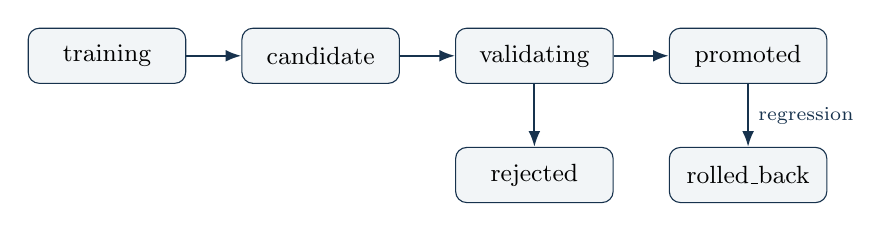
\begin{tikzpicture}[
    state/.style={draw=PaperBlue, rounded corners, fill=PaperLight, minimum width=2.0cm,
      minimum height=7mm, align=center, font=\small},
    arrow/.style={-{Latex[length=2mm]}, thick, color=PaperBlue},
    node distance=8mm and 7mm
  ]
    \node[state] (training) {training};
    \node[state, right=of training] (candidate) {candidate};
    \node[state, right=of candidate] (validating) {validating};
    \node[state, right=of validating] (promoted) {promoted};
    \node[state, below=of validating] (rejected) {rejected};
    \node[state, below=of promoted] (rollback) {rolled\_back};
    \draw[arrow] (training) -- (candidate);
    \draw[arrow] (candidate) -- (validating);
    \draw[arrow] (validating) -- (promoted);
    \draw[arrow] (validating) -- (rejected);
    \draw[arrow] (promoted) -- node[right,font=\scriptsize]{regression} (rollback);
  \end{tikzpicture}
  \caption{不可变 Policy Version 的生命周期；训练完成只是 candidate，不等于晋升。}
\end{figure}

\section{Qwen3.6 27B、H200 与 vLLM 分层}

训练后端、服务后端和控制面必须分开。H200 存储冻结 Qwen base、optimizer/LoRA checkpoint 和 immutable exported
adapter；PyTorch/PEFT/TRL/verl 承担训练；vLLM/OpenAI-compatible endpoint 承担推理；ScienceFlow Registry
承担版本与路由。

训练进程不得覆盖 vLLM 正在读取的 adapter 目录。导出使用临时目录、SHA 校验和原子 rename；promotion 前执行
readiness probe，失败时 active endpoint 不变。用户指定的“Qwen3.6 27B”必须在运行 manifest 中解析为精确
model ID、weight SHA、tokenizer SHA、serving revision 和 sampling config，简称不能成为复现依据。

资源上，Agent inference、Evaluator GPU 和 Learner 分别声明 resource class。Learner 默认低于交互式 inference；
显存不足时 checkpoint/pause learner，不杀有 pending effect 的 Agent。远端 H200 保存大对象，本地 Workspace
保存 manifest 与 SHA；Resume 只恢复逻辑 lease，物理 GPU 占用重新验证。

\section{组件边界与配置}

实现不增加新的 ScienceFlow 顶层目录。typed records/ports 放在 foundation contracts；experience、objective、
policy、resume 放在 research learning；trainer、process、serving、resource effect 放在 runtime learning；CLI 只
调用公开 service。每个目录继续满足不超过五个直接子目录/业务模块的门禁。

\begin{table}[htbp]
  \centering
  \caption{建议组件及唯一职责}
  \begin{tabularx}{\textwidth}{@{}L{3.0cm}YY@{}}
    \toprule
    组件 & 拥有 & 不拥有 \\
    \midrule
    Experience Service & eligibility、record、dedup、cursor & factual Memory、Workspace effect \\
    Objective Service & advantage、KL、batch decision & trainer process、GPU lease \\
    Learner Runtime & backend lifecycle、checkpoint、export & promotion policy \\
    Policy Registry & immutable version、CAS、routing cursor & evaluator 算法 \\
    Promotion Service & shadow/bench evidence、decision & 直接覆盖服务目录 \\
    Composite Checkpoint & participant barrier、audit & 各 participant 内部状态机 \\
    Serving Adapter & readiness、load/switch/rollback effect & candidate quality decision \\
    \bottomrule
  \end{tabularx}
\end{table}

默认配置必须是 \code{ttt.enabled=false}。V1 推荐 semi-async、task scope、LoRA rank 32、Stage boundary、
max policy lag 1、authoritative reward、adaptive entropic advantage、parent KL 0.1、每 batch checkpoint、两次
bench Resume 和禁止 mid-stage switch。所有数值都是初始配置，不是已验证最优值。

\section{失败模式和安全裁决}

\begin{longtable}{L{3.4cm}L{5.3cm}L{5.0cm}}
  \caption{关键失败模式、正确恢复与禁止行为}\label{tab:failure}\\
  \toprule
  失败 & 正确裁决 & 禁止行为 \\
  \midrule
  \endfirsthead
  \toprule
  失败 & 正确裁决 & 禁止行为 \\
  \midrule
  \endhead
  Tool Call 后 Actor 崩溃 & pending effect reconciliation，按 effect ID 裁决 & 重新生成整个 assistant turn \\
  Experience 重复投递 & trajectory content ID 去重 & 重复进入同一 batch \\
  backward 后 Learner 崩溃 & 回前一 committed checkpoint，重算整批 & 猜测 optimizer 是否执行 \\
  Adapter 导出不完整 & candidate rejected，active 不变 & 覆盖 active adapter \\
  Promotion 写入后崩溃 & CAS/operation ID 判断已提交 & 再次递增版本或重复切换 \\
  Reward contract 改变 & 旧经验 quarantine、新 queue & 静默混训 \\
  Policy lag 超限 & discard/requeue 并记录原因 & 当作当前 on-policy 样本 \\
  H200 不可达 & Agent 继续 current promoted policy & 阻塞所有 Agent \\
  vLLM readiness 失败 & 保持 parent endpoint & 晋升不可服务版本 \\
  五域 cursor 不一致 & 拒绝 composite checkpoint & 各域分别选择最新文件 \\
  GPU lease owner 死亡 & stale reconciliation 后重新 admission & 继承旧 PID 或物理占用 \\
  Reward 异常升高 & hacking audit、held-out verifier & 只看单次最高分晋升 \\
  \bottomrule
\end{longtable}

主要安全风险是 reward hacking、数据泄漏、灾难性遗忘、训练数据污染和资源抢占。控制手段包括 held-out verifier、
artifact validation、provenance/retention policy、task adapter、quarantine、resource priority、safe preemption 和
人工可回滚的 allowlist。Online autonomous promotion 必须晚于手工 promotion 稳定阶段。

\section{验证设计}

\subsection{单元、合同与 Runtime Parity}

单元/合同测试覆盖 schema/hash、eligibility/redaction/dedup、advantage/KL、Registry CAS、barrier prepare/commit/
abort、stale trajectory、constant reward、contract drift 和 package dependency。TTT 关闭时现有 provider context、
Tool schema、event ordering 和 Workspace effect 必须零漂移；capture-only 只允许新增登记的 learning telemetry/object。

\subsection{bench\_sf Resume Cases}

\begin{longtable}{L{4.0cm}L{4.4cm}L{5.4cm}}
  \caption{TTT V1 建议新增的真实 Resume Case}\label{tab:bench}\\
  \toprule
  Case & Resume 边界 & 硬 Oracle \\
  \midrule
  \endfirsthead
  \toprule
  Case & Resume 边界 & 硬 Oracle \\
  \midrule
  \endhead
  \nolinkurl{ttt_experience_commit} & Gate accepted、append 前 & trajectory 单次提交、reward/source SHA 一致 \\
  \nolinkurl{ttt_learner_batch} & optimizer step 周边 & committed 不重做、半步不误认 \\
  \nolinkurl{ttt_workspace_policy_atomic} & provisional barrier 后 & 五域 cursor 同一 barrier \\
  \nolinkurl{ttt_stale_trajectory} & old-policy item 已排队 & lag 裁决确定、不得训练 \\
  \nolinkurl{ttt_policy_promotion} & validated、CAS 前 & 单次 promotion、active pointer 正确 \\
  \nolinkurl{ttt_stage_boundary_switch} & 新版 promoted、旧 Stage 未结束 & 旧 Stage pin，新 Stage 使用新版本 \\
  \nolinkurl{ttt_policy_rollback} & regression 触发、回滚前 & parent 恢复、candidate 保留审计 \\
  \nolinkurl{ttt_reward_contract_drift} & reward version 更新 & 旧经验 quarantine、不混 batch \\
  \nolinkurl{ttt_h200_learner_recovery} & remote learner 中断 & stale lease 清理、checkpoint 可加载 \\
  \nolinkurl{ttt_vllm_readiness} & adapter 导出、服务切换前 & readiness 失败不影响 active \\
  \bottomrule
\end{longtable}

每个 stable case 必须从同一只读 bundle 做两次独立 Resume。模型文本不要求逐字一致；event ordering、状态原子性、
effect 去重、artifact SHA 和资源清理是硬门禁。发布候选再执行 Circle、Nomad、TFBind8 从零长程矩阵，对比
frozen parent、capture-only、train-no-promotion 和 auto-promotion，并报告未触发、失败和环境错误。

\section{分阶段实施计划}

\begin{table}[htbp]
  \centering
  \caption{TTT V1 实施阶段及完成条件}
  \begin{tabularx}{\textwidth}{L{1.3cm}L{3.3cm}YY}
    \toprule
    阶段 & 主题 & 主要交付 & 完成条件 \\
    \midrule
    V1-0 & 合同与 Capture & typed records、hash、projector、NOTICE & 真实 Stage 产生脱敏可审计 Experience \\
    V1-1 & 离线 Learner & Qwen+PEFT、objective、batch/checkpoint & 固定经验可重放恢复，不接 online routing \\
    V1-2 & Composite Resume & participants、barrier、audit、bench & 四类中断无重复 effect/step \\
    V1-3 & H200 半异步 & remote learner、resource、export、readiness & 后台产生 candidate，故障不阻塞 Agent \\
    V1-4 & 人工晋升 & Registry、shadow/bench、CLI、Stage router & 仅新 Stage 使用 promoted policy \\
    V1-5 & 自动闭环 & auto gate、online rollback、ESTRA routing & allowlist 内无人工闭环可审计 Resume \\
    V1-6 & Full Async & 多版本 queue、off-policy、dynamic batch & 单独验收，不包含 base merge \\
    \bottomrule
  \end{tabularx}
\end{table}

第一步应是 V1-0，而非直接训练：建立 TrajectoryRecord、RewardContract、PolicyVersion 和
CompositeCheckpointManifest，以 capture-only 从 Circle 或现有 bench checkpoint 产生真实 Experience。先发现
provenance、脱敏、effect pairing 和 reward 定义错误，再消耗 H200 训练资源。

\section{完成定义与待决策项}

V1 完成必须同时满足：上游许可和差异记录完整；Qwen LoRA 在 H200 实际训练并 Resume；执行与训练真实异步；
Composite Checkpoint 覆盖五域；policy version 在 provider/Stage/trajectory/artifact 可追踪；promotion/rollback
幂等且边界正确；reward 权威并有 drift/hacking gate；TTT bench 每项两次独立 Resume；TTT disabled parity 零漂移；
至少一个真实任务自动完成 experience--train--validate--promote/rollback；Circle/Nomad/TFBind8 发布矩阵报告完整；
操作、清理和回滚文档齐全。

实现前必须冻结 Qwen3.6 27B 的精确 checkpoint/tokenizer、训练 backend、vLLM LoRA readiness、首个 task/reward、
promotion 非劣阈值、experience 许可/保留周期、adapter 对象存储以及自动 promotion allowlist。

\section{结论}

ScienceFlow 现有 Workspace/Stage/Memory/Resource Resume 为 TTT-Discover 缺失的 agentic 长程一致性提供了合适基础。
可行路线不是把同步训练函数嵌入 Agent，也不是直接热改全量 Qwen，而是构建版本化 Actor--Learner：Actor pin 到
不可变 policy，Learner 异步训练 task LoRA，Composite Checkpoint 绑定五类状态，candidate 经 shadow 和真实
Resume 后在 Stage/lineage 边界晋升。该设计可以实现自主迭代，同时保留可解释、可回滚和可复现边界。真正完成
仍需 H200 实训、TTT 专属 bench 以及正式长程矩阵证据。

\section*{数据、构建与复现说明}

Canonical 工程规划位于 \nolinkurl{docs/ttt/plan_v1/plan_v1.md}；本文 LaTeX 源稿位于同目录
\nolinkurl{ttt_scienceflow_plan_v1.tex}。构建命令如下：

\begin{center}
\small\ttfamily
tectonic --keep-logs --keep-intermediates\\
ttt\_scienceflow\_plan\_v1.tex
\end{center}
本文没有使用实验数据或生成统计图；所有表格来自源码审计和设计合同。后续实验必须将 manifest、raw event、
scorecard、模型/数据 SHA 和负面结果保存在用户指定的独立运行目录。

\begin{thebibliography}{9}
\bibitem{ttt-paper}
M. Yuksekgonul et al., ``Learning to Discover at Test Time,''
\emph{arXiv preprint arXiv:2601.16175}, 2026.

\bibitem{ttt-repo}
Test-Time Training Project, ``TTT-Discover,'' commit \nolinkurl{6c40e82},
MIT License, 2026.
\url{https://github.com/test-time-training/discover}.

\bibitem{sf-bench}
ScienceFlow Project, ``bench\_sf V1: ScienceFlow 可恢复长程技术基准,''
\nolinkurl{docs/benchmark/bench_sf_v1.md}, 2026.

\bibitem{sf-memory}
ScienceFlow Project, ``Memory 与 ESTRA 架构,''
\nolinkurl{docs/architecture/memory_estra_v3.md}, 2026.

\bibitem{sf-resource}
ScienceFlow Project, ``Resource Management 架构,'' 2026.\newline
\nolinkurl{docs/architecture/resource_management_v3.md}.
\end{thebibliography}

\end{document}
